\documentclass{article}
\usepackage[margin=2cm]{geometry}
\usepackage{graphicx}
\usepackage{subcaption}
\usepackage{tabu}
\usepackage{mathtools}
%\usepackage{amsmath}
% \graphicspath{ {Q1/images/}{Q2/images/}{Q3/images/}{Q4/images/} }
\title{COL783 Assignment 2}
\date{}
\author{Lovish Madaan \\ \texttt{2015CS50286} \and Nikhil Goyal \\ \texttt{2015CS50287}}
\begin{document}
\maketitle
\section{Face Morphing}
\subsection{Approach}
\begin{itemize}
    \item Established correspondence of features using dlib's automatic facial landmark detection. Additional points can be provided by the user.
    \item Used Delaunay triangulation to obtain the triangulation of feature points.
    \item Transformed the corresponding feature triangles of the input images to the destination image feature triangle using Barycentric coordinates.
\end{itemize}

\subsection{Results}
\begin{figure}[!ht]
\begin{subfigure}{.33\textwidth}
\centering
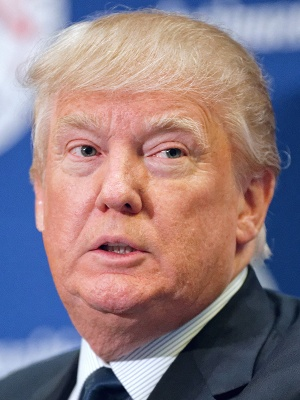
\includegraphics[width=.75\linewidth]{m00.jpg}
\end{subfigure}
\begin{subfigure}{.33\textwidth}
\centering
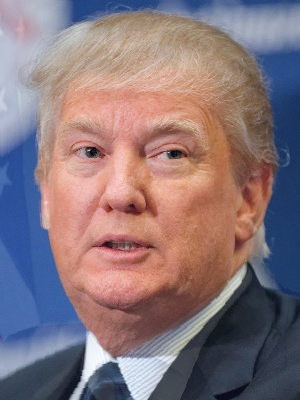
\includegraphics[width=.75\linewidth]{m02.jpg}
\end{subfigure}
\begin{subfigure}{.33\textwidth}
\centering
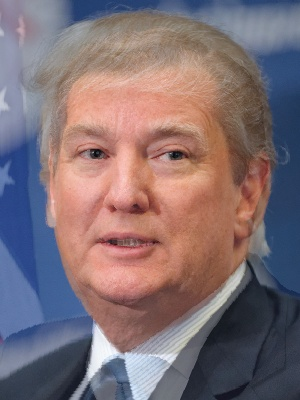
\includegraphics[width=.75\linewidth]{m04.jpg}
\end{subfigure}
\begin{subfigure}{.33\textwidth}
\centering
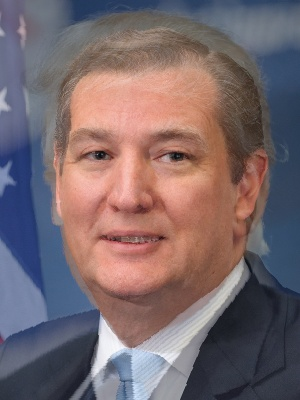
\includegraphics[width=.75\linewidth]{m06.jpg}
\end{subfigure}
\begin{subfigure}{.33\textwidth}
\centering
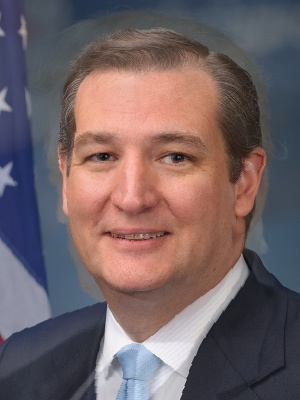
\includegraphics[width=.75\linewidth]{m08.jpg}
\end{subfigure}
\begin{subfigure}{.33\textwidth}
\centering
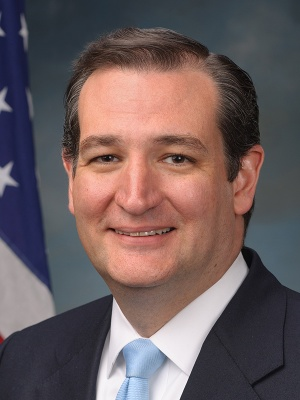
\includegraphics[width=.75\linewidth]{m10.jpg}
\end{subfigure}
\caption{Face Morphing}
\end{figure}

\clearpage

\section{Face Swapping}
\subsection{Approach}
\begin{itemize}
    \item Similar to the face morphing approach, corresponding feature points were obtained for only the portion of the face to be swapped.
    \item Computed convex hull followed by delaunay triangulation to get the novice image(simply swapped).
    \item Implemented local gaussian blurring to change the coloring of the image. We did it by dividing the source image by the gaussian blur of second image followed by multiplication with gaussian blur of source image.
    \item Implemented Seamless Cloning for colour correction and boundary smoothing using finite difference approximation and conjugate gradient method to solve the matrix equation.
    \item Used alpha blending for the final image to reduce sharp boundaries.
\end{itemize}

\subsection{Results}

\begin{figure}[!ht]
\begin{subfigure}{.24\textwidth}
\centering
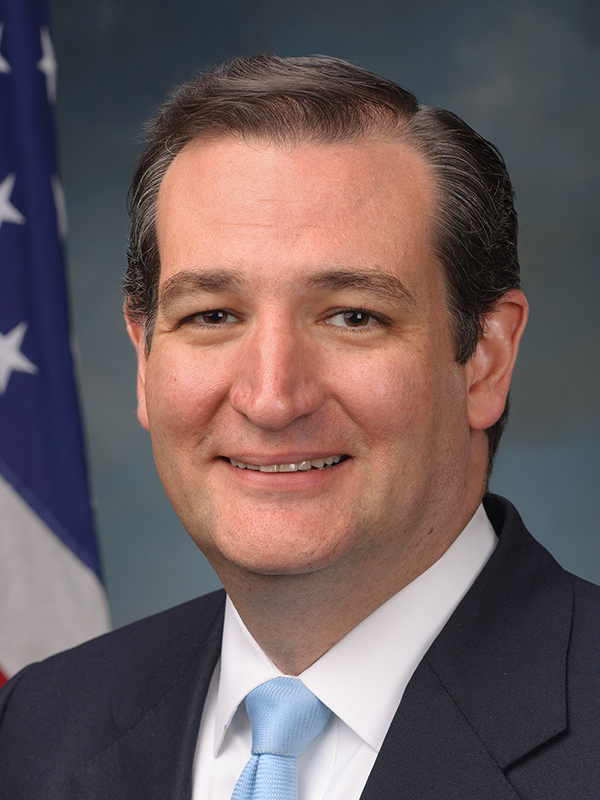
\includegraphics[width=.75\linewidth]{ted_cruz.jpg}
\caption{Image 1}
\end{subfigure}
\begin{subfigure}{.24\textwidth}
\centering
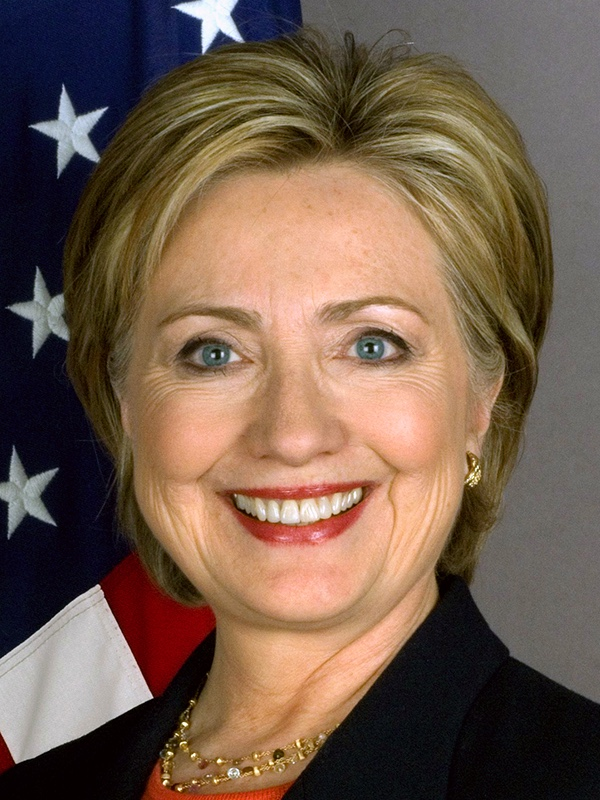
\includegraphics[width=.75\linewidth]{hillary_clinton.jpg}
\caption{Image 2}
\end{subfigure}
\begin{subfigure}{.24\textwidth}
\centering
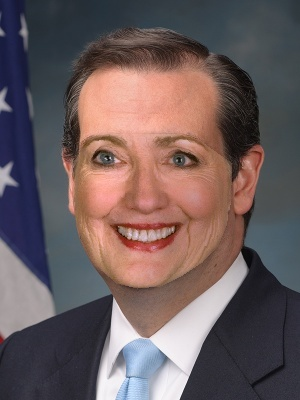
\includegraphics[width=.75\linewidth]{gaussian1.jpg}
\caption{Gaussian Blur}
\end{subfigure}
\begin{subfigure}{.24\textwidth}
\centering
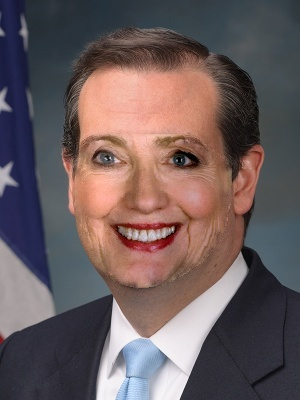
\includegraphics[width=.75\linewidth]{seamless1.jpg}
\caption{Seamless Cloning}
\end{subfigure}
\caption{Face Swapping 1}
\end{figure}

\begin{figure}[!ht]
\begin{subfigure}{.24\textwidth}
\centering
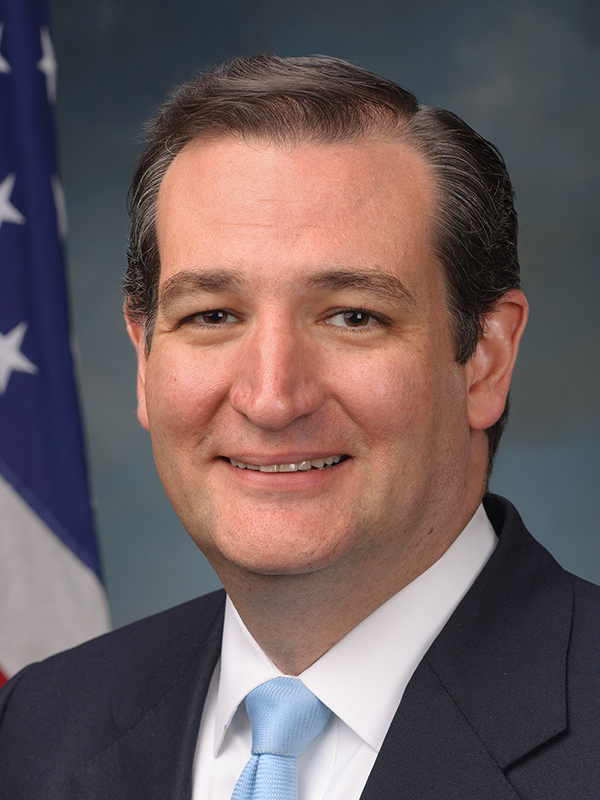
\includegraphics[width=.75\linewidth]{ted_cruz.jpg}
\caption{Image 1}
\end{subfigure}
\begin{subfigure}{.24\textwidth}
\centering
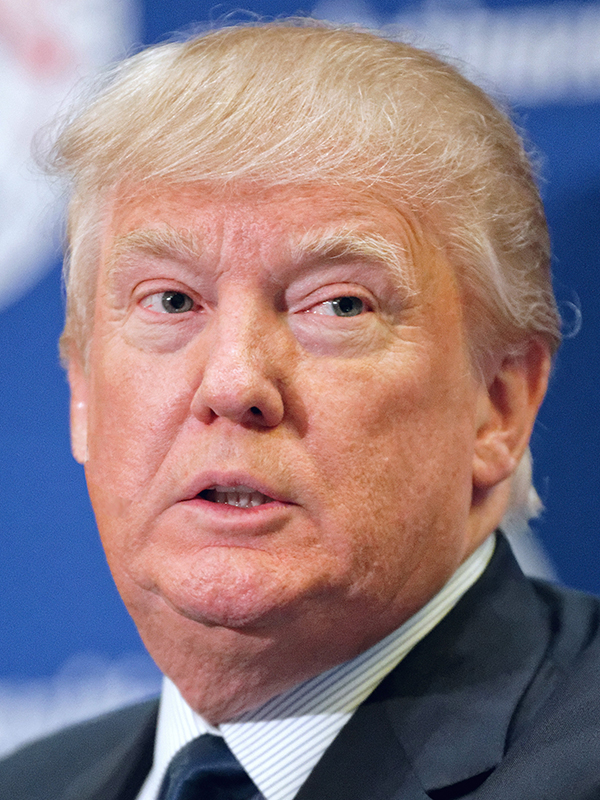
\includegraphics[width=.75\linewidth]{donald_trump.jpg}
\caption{Image 2}
\end{subfigure}
\begin{subfigure}{.24\textwidth}
\centering
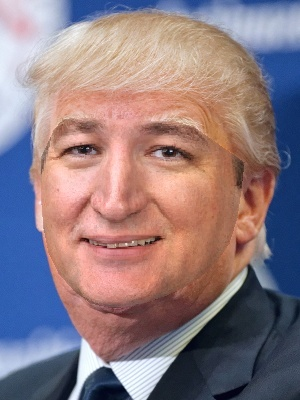
\includegraphics[width=.75\linewidth]{gaussian2.jpg}
\caption{Gaussian Blur}
\end{subfigure}
\begin{subfigure}{.24\textwidth}
\centering
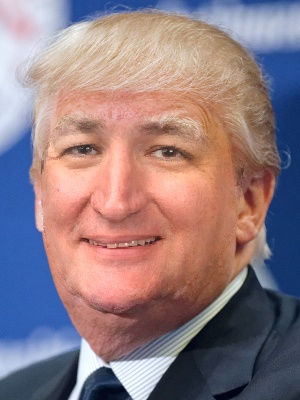
\includegraphics[width=.75\linewidth]{seamless2.jpg}
\caption{Seamless Cloning}
\end{subfigure}
\caption{Face Swapping 2}
\end{figure}

\clearpage

\section{Filters for augmenting face}
\subsection{Approach}
\begin{itemize}
    \item Used three filters - moustache, eye mask and jaw cover filter.
    \item Used dlib's automatic feature extractor to get the face landmarks.
    \item Used affine transformation/perspective transformation to map the filter to the corresponding feature points and then used alpha blending to get the final image.
\end{itemize}

\subsection{Results}

\begin{figure}[!ht]
\begin{subfigure}{.5\textwidth}
\centering
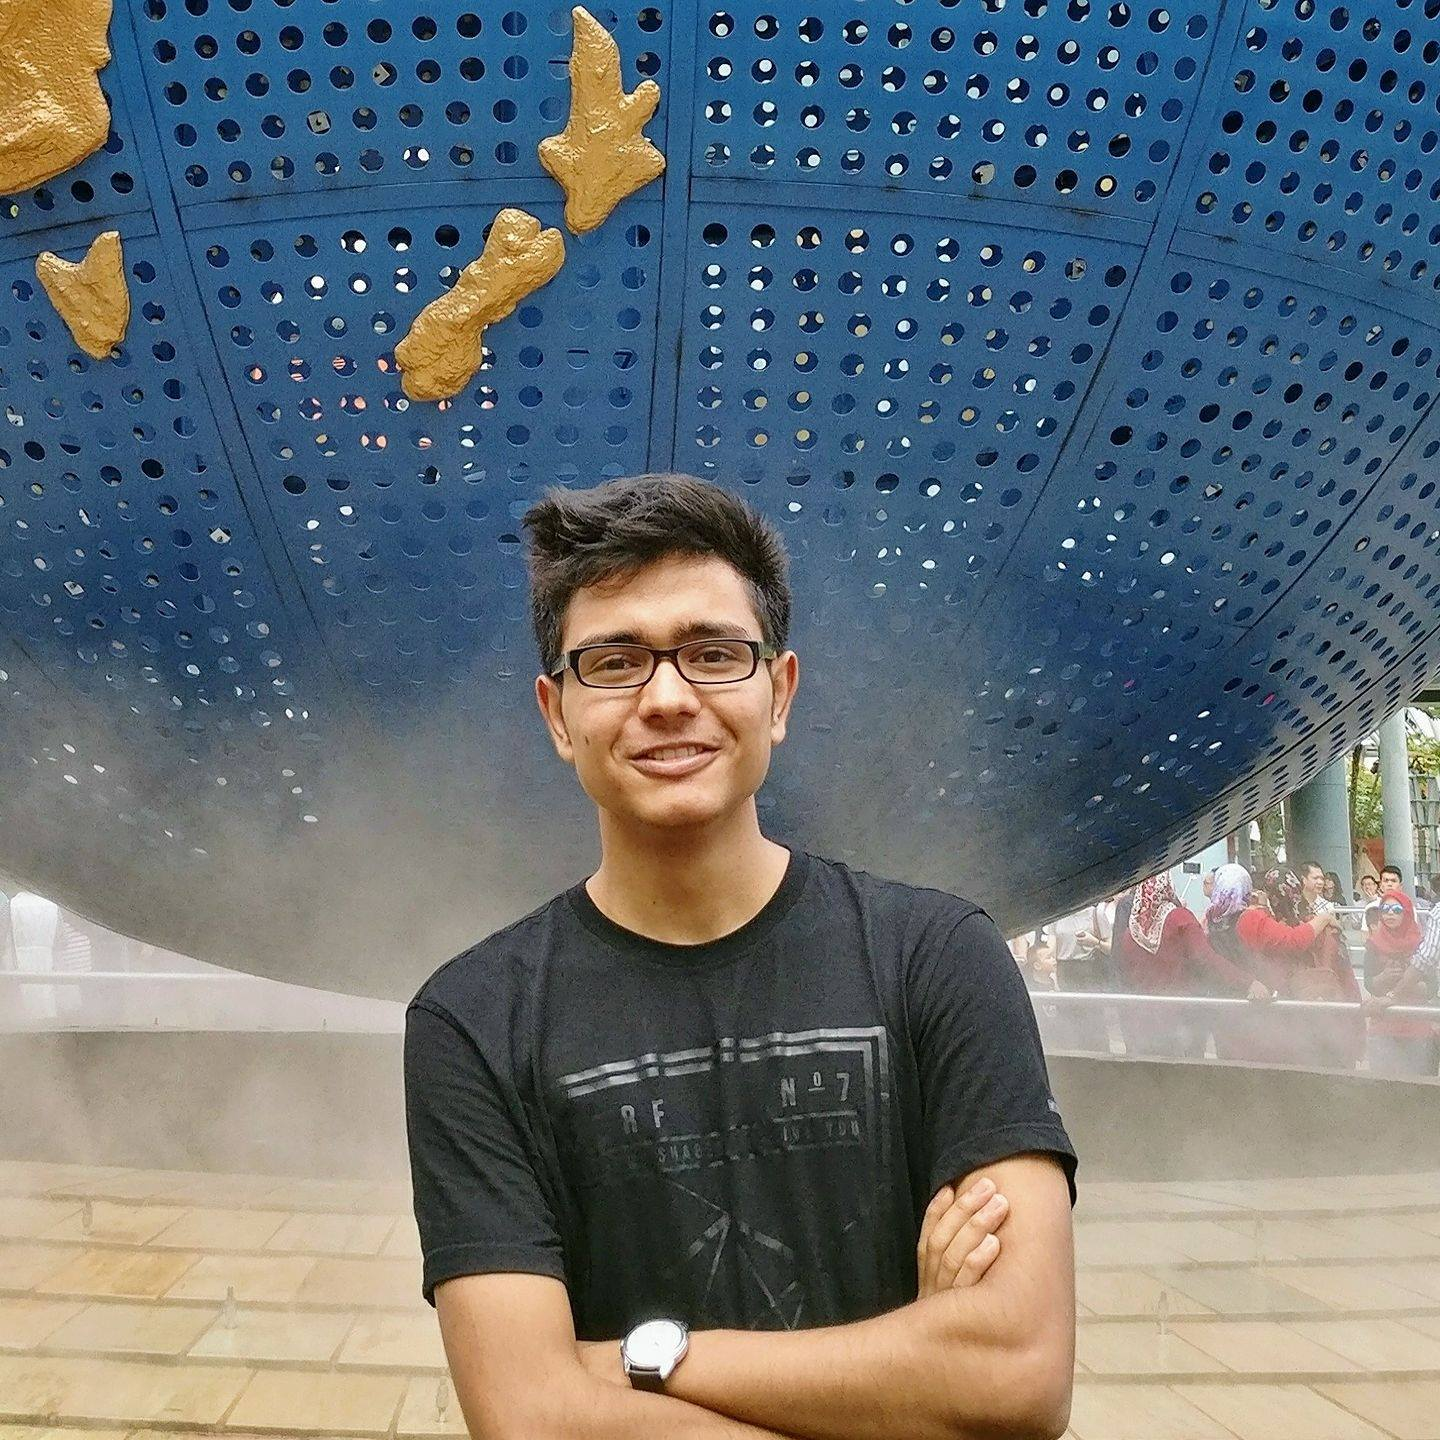
\includegraphics[width=.75\linewidth]{c3.JPG}
\caption{Original Image}
\end{subfigure}
\begin{subfigure}{.5\textwidth}
\centering
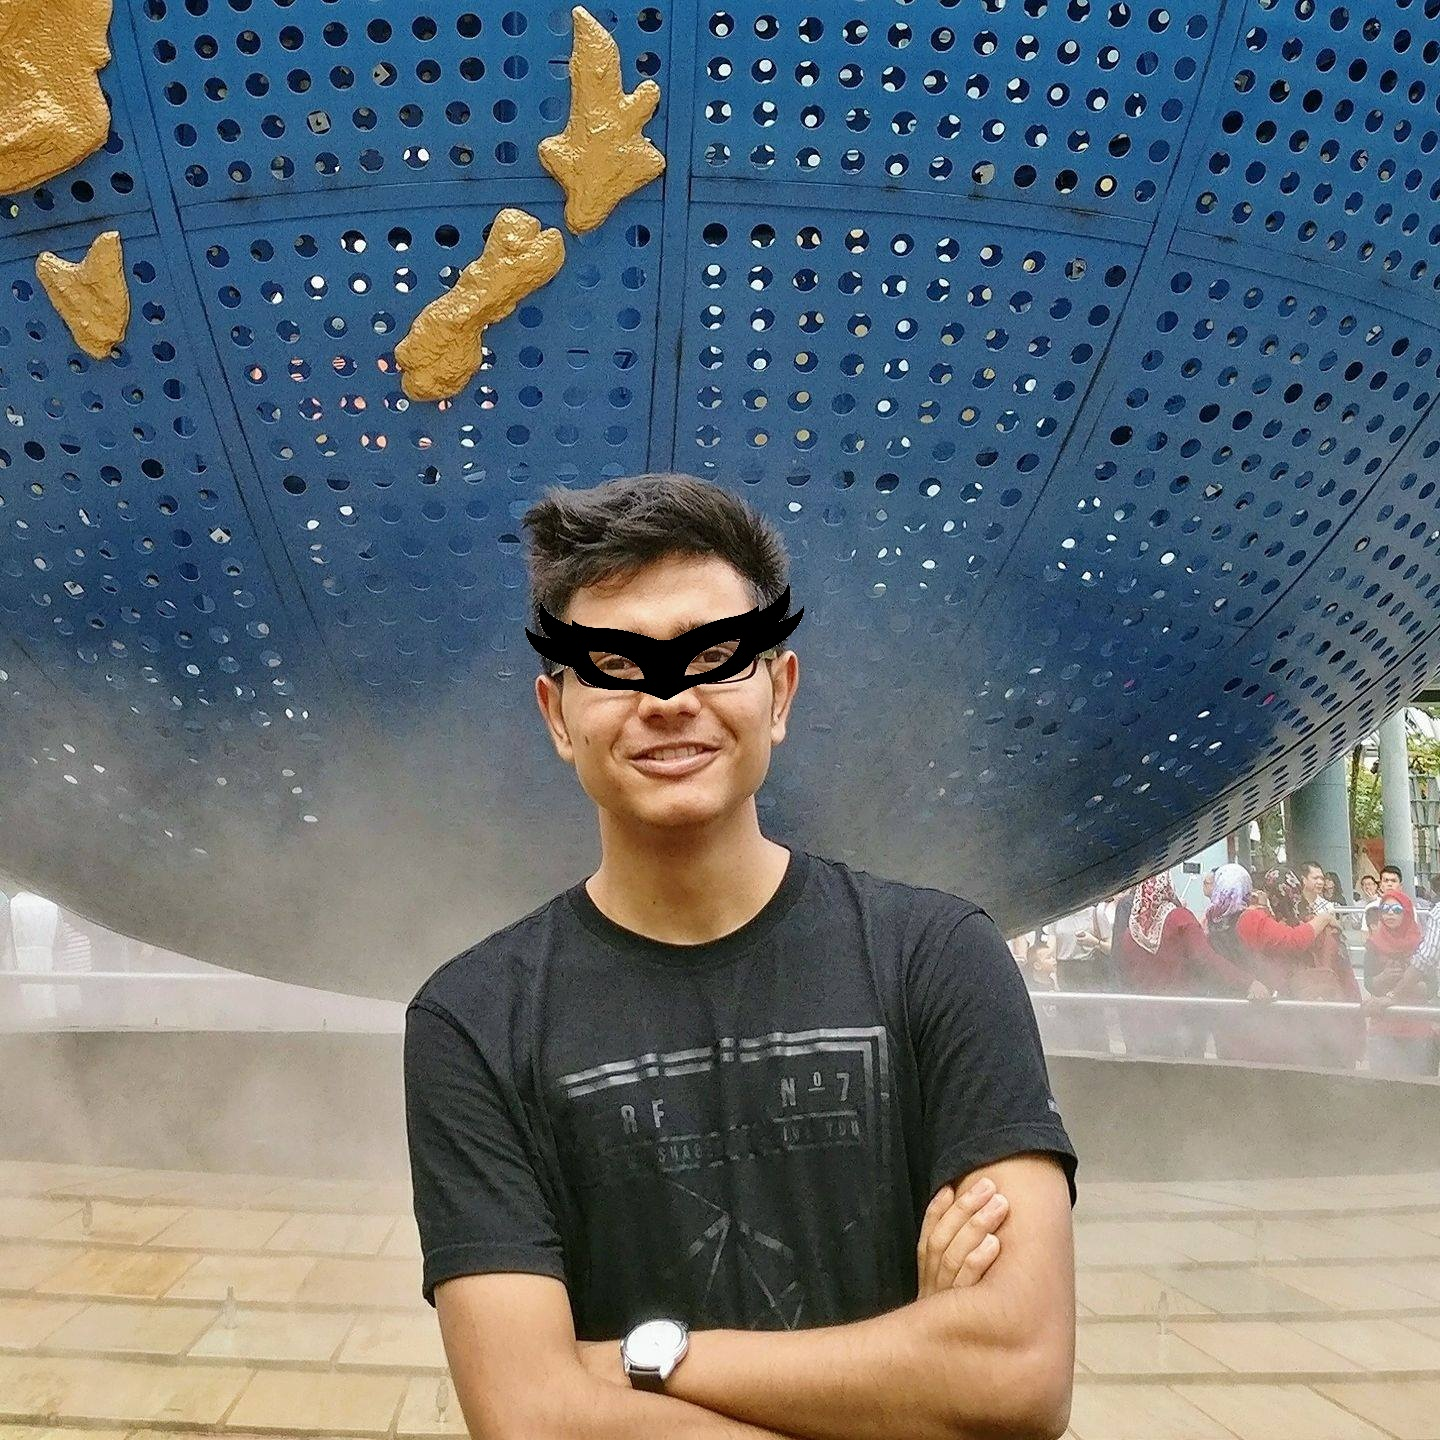
\includegraphics[width=.75\linewidth]{eye_mask.jpg}
\caption{Eye Mask Filter}
\end{subfigure}
\begin{subfigure}{.5\textwidth}
\centering
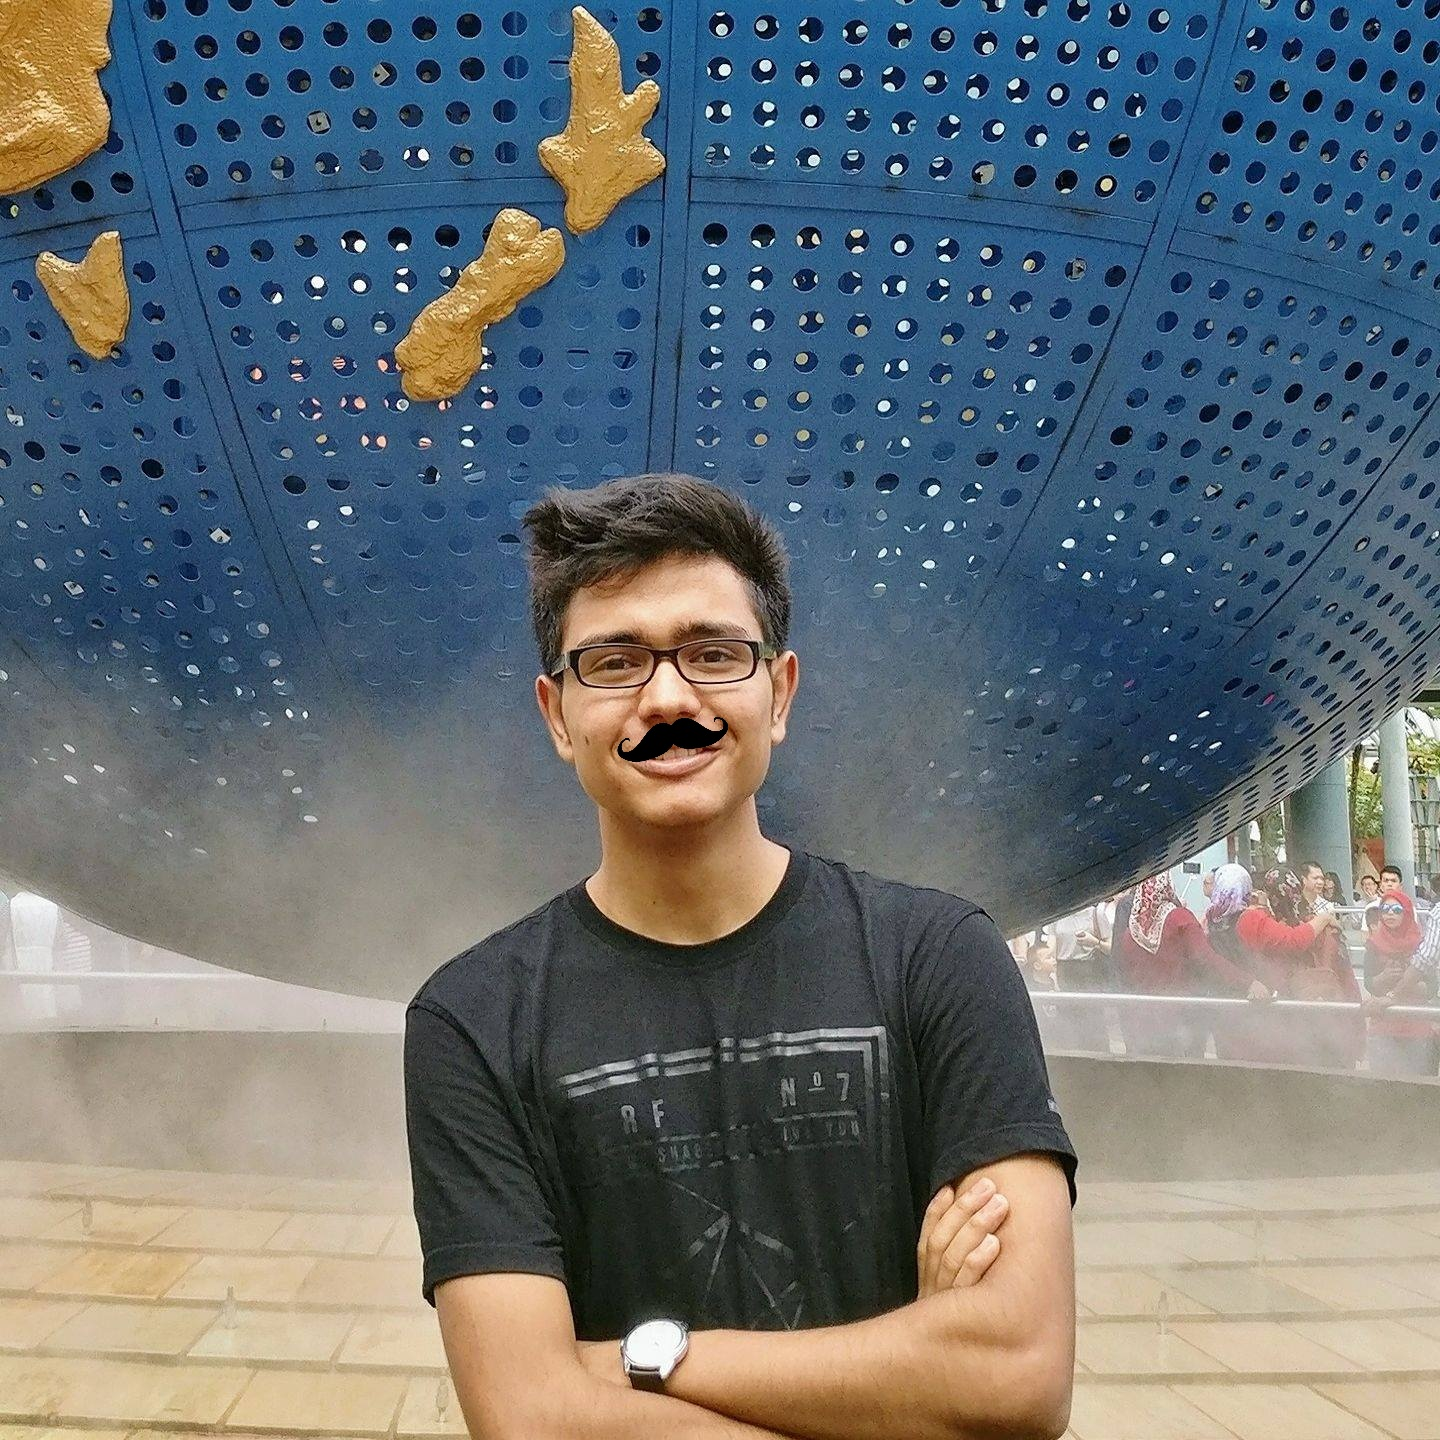
\includegraphics[width=.75\linewidth]{muchan.jpg}
\caption{Moustache Filter}
\end{subfigure}
\begin{subfigure}{.5\textwidth}
\centering
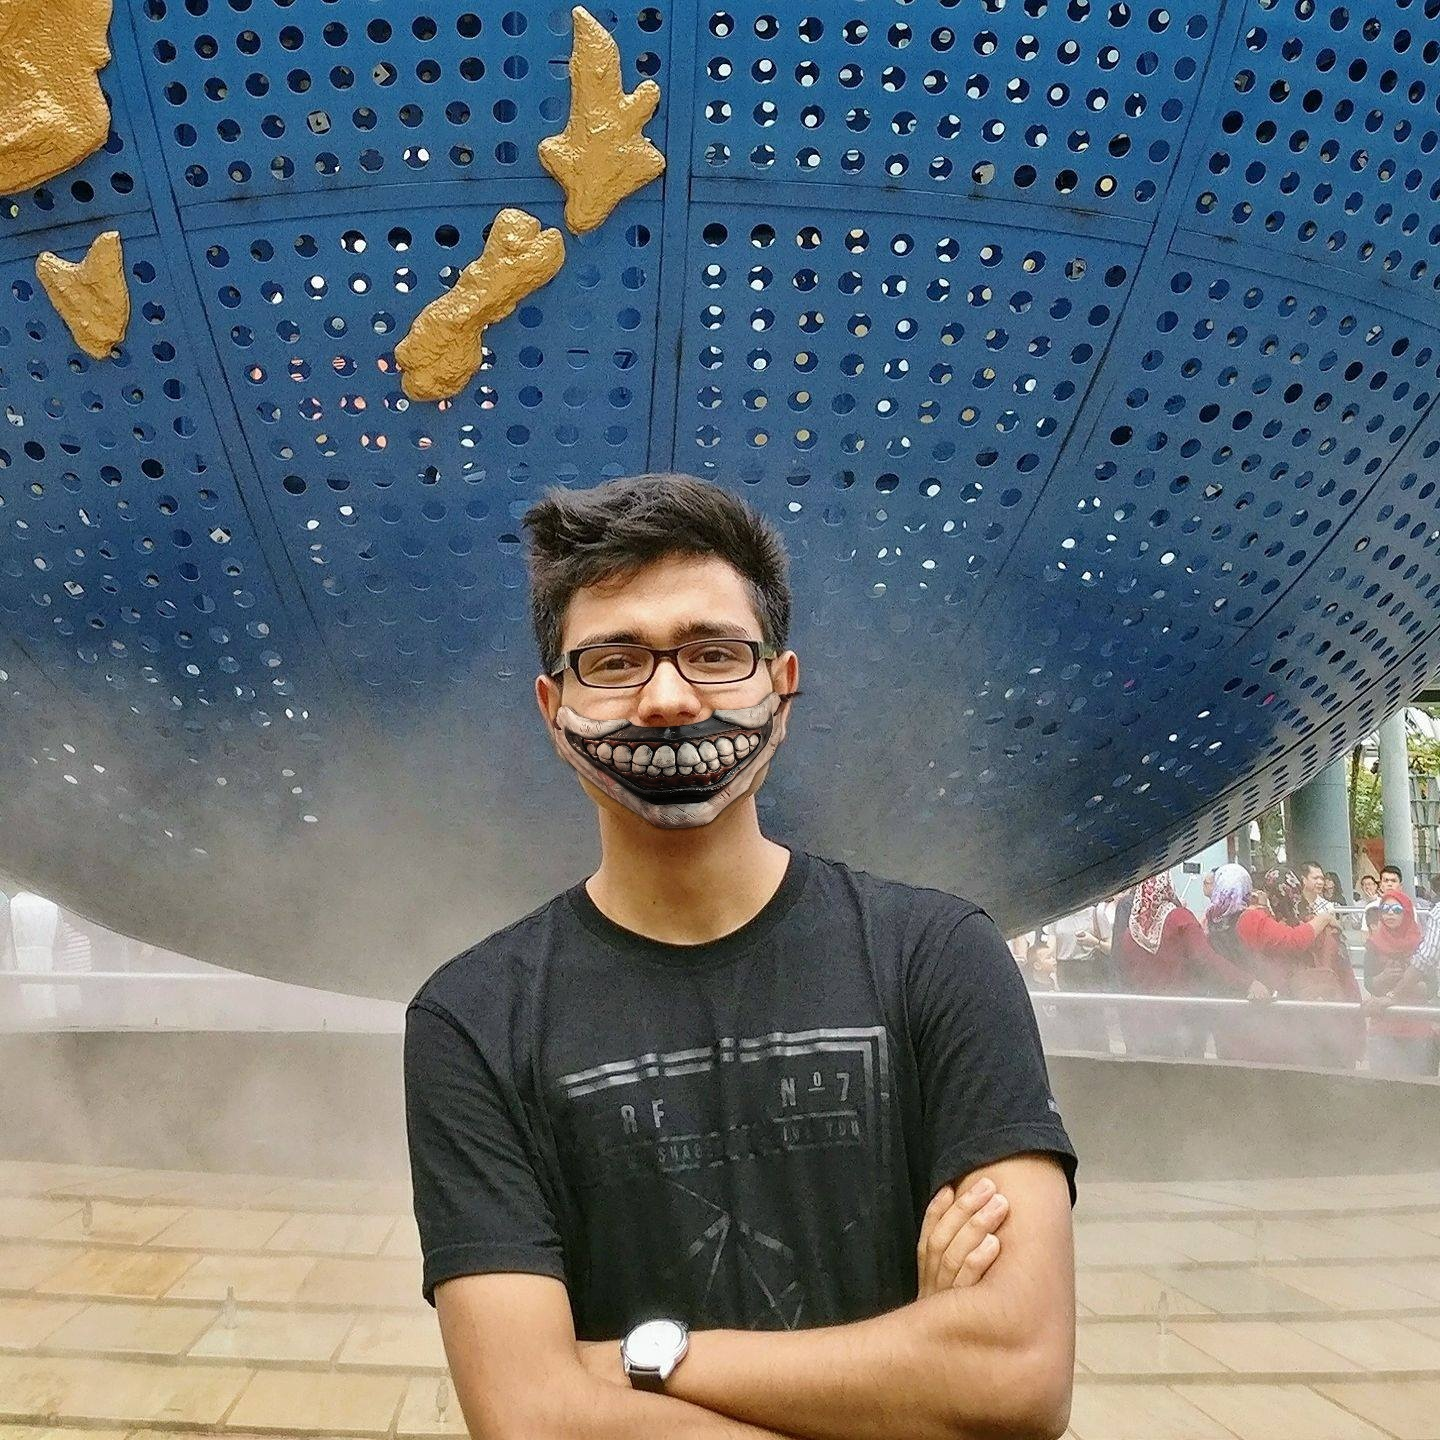
\includegraphics[width=.75\linewidth]{jaws.jpg}
\caption{Jaws Filter}
\end{subfigure}
\caption{Part 3}
\end{figure}

\end{document}